%--------------------------------------------------------------------------------------------------------------------
%------------------------------------------------- Appendix A ---------------------------------------------------------
%\addcontentsline{toc}{chapter}{Ap{\'e}ndices}
\renewcommand{\thesection}{A.\arabic{section}}
\renewcommand{\theequation}{a.\arabic{equation}}
\renewcommand{\thefigure}{A.\arabic{figure}}
%\setcounter{section}{0}
%\setcounter{equation}{0}

\chapter{Ap{\'e}ndices}
\section{MCR con factor de olvido}\label{A_1}
Recordando el criterio de minimizaci{\'o}n de la ec. \ref{e2_29}, podemos considerar un pesado exponencial para
el error de predicci{\'o}n
\begin{equation}
  V_N\left(\theta,Z^N\right)=\frac{1}{N}\sum_{k=1}^{N}\lambda^{N-k}\left(y(k)-\varphi(k)^T\theta\right)^2
\end{equation}
con $0<\lambda\leq1$, as{\'\i} resulta que los datos mas nuevos ($\lambda^{N-k}$ cercano a 1) ser{\'a}n tratados con
mayor importancia en el funcional, por otro lado los datos mas viejos ($\lambda^{N-k}$ cercano a 0) ser{\'a}n
olvidados dentro del criterio.

Para este caso la estima de m{\'\i}nimos cuadrados resulta
\begin{equation}\label{a_2}
\hat{\theta}_N=\left[\sum_{k=1}^{N}\lambda^{N-k}\varphi(k)\varphi(k)^T\right]^{-1}\sum_{k=1}^{N}\lambda^{N-k}\varphi(k)y(k)
\end{equation}
denominado ahora con
\begin{equation}\label{a_3}
    P_{N}=\left[\sum_{k=1}^{N}\lambda^{N-k}\varphi(k)\varphi(k)^T\right]^{-1}
\end{equation}
se puede expresar que
\begin{equation}
    P^{-1}_{N}=\sum_{k=1}^{N}\lambda^{N-k}\varphi(k)\varphi(k)^T=
               \sum_{k=1}^{N-1}\lambda^{N-k}\varphi(k)\varphi(k)^T+\varphi(N)\varphi(N)^T
\end{equation}
notar que en este caso se puede expresar $\lambda^{N-k}=\lambda^{N-k-1}\lambda$, resultando en
\begin{equation}
    P^{-1}_{N}=\lambda\left[\sum_{k=1}^{N-1}\lambda^{N-k-1}\varphi(k)\varphi(k)^T\right]+\varphi(N)\varphi(N)^T=
               \lambda P^{-1}_{N-1}+\varphi(N)\varphi(N)^T
\end{equation}
La estima de m{\'\i}nimos cuadrados para $N$ datos entrada-salida puede expresarse como
\begin{equation}
\begin{split}
\hat{\theta}_{N}=&P_{N}\left[\lambda\sum_{k=1}^{N-1}\lambda^{N-k-1}\varphi(k)y(k)+\varphi(N)y(N)\right]\\
                =&P_{N}\left[\lambda P_{N-1}^{-1}\hat{\theta}_{N-1}+\varphi(N)y(N)\right]\\
                =&P_{N}\lambda \left[\frac{P_N^{-1}-\varphi(N)\varphi(N)^T}{\lambda}\right]\hat{\theta}_{N-1}+P_N\varphi(N)y(N)\\
                =&\hat{\theta}_{N-1}+P_{N}\varphi(N)\left[y(N)-\varphi(N)^T\hat{\theta}_{N-1}\right]
\end{split}
\end{equation}
que resulta igual a el caso sin factor de olvido.

Considerando ahora $A=\lambda P_{N-1}^{-1}$, $B=\varphi(N)$, $C=\varphi(N)^T$ y $D=1$ para el lema de
inversi{\'o}n de matrices, resulta que en este caso debe ser
\begin{equation}
      P_{N}=\frac{1}{\lambda}\left[P_{N-1}-\frac{P_{N-1}\varphi(N)\varphi(N)^TP_{N-1}}{\lambda+\varphi(N)^TP_{N-1}\varphi(N)}\right]
\end{equation}

\section{Predicci{\'o}n con modelo FIR}\label{A_2}
De esta forma, considerando el error planta-modelo $\eta(k)$ (estimaci{\'o}n de perturbaciones) las predicciones
del modelo vienen dadas por
\begin{equation}
\begin{split}
\hat{y}(k+i) &= \sum_{j=1}^{N}g(j)u(k+i-j) + \eta(k+i)\\
             &= \underbrace{\sum_{j=1}^{i}g(j)u(k+i-j)}_{\text{acciones futuras}}+
                \underbrace{\sum_{j=i+1}^{N}g(j)u(k+i-j)}_{\text{acciones pasadas}}+ \eta(k+i)
\end{split}
\end{equation}
donde $u(k+i)$ es la se{\~n}al de control y $\hat{y}(k+i)$ la predicci{\'o}n del modelo. Una forma simple de obtener
una estimaci{\'o}n de la perturbaci{\'o}n (error planta-modelo) es considerarla constante sobre todo el intervalo de
predicci{\'o}n, $\eta(k+i)=\eta(k)=y(k)-\hat{y}(k)$ para $i=H_w,\ldots,H_p$.

Las predicciones del modelo en el horizonte $[H_w,H_p]$ pueden expresarse como la superposici{\'o}n de dos
efectos, por un lado las acciones pasadas de control contenidas en $\psi(k)$ y los efectos de las acciones
futuras de control referidas con $\mathbf{\hat{u}}(k)$, es decir:
\begin{equation}
    \hat{\mathbf{y}}(k)=\mathbf{T}_{1}\mathbf{GT}_{2}\mathbf{\hat{u}}(k)+
                        \mathbf{T}_{3}\mathbf{ST}_{4}\mathbf{\psi}(k)+
                        \mathbf{\hat{\eta}}(k)
\end{equation}
con
\begin{align}
         \hat{\mathbf{y}}(k) & = \left[\hat{y}(k+H_w),\cdots,\hat{y}(k+H_p)\right]^{T}   \\
      \mathbf{\hat{\eta}}(k) & = \left[1,\cdots,1\right]^{T}\left[y(k)-\hat{y}(k)\right] \\
         \mathbf{\hat{u}}(k) & = \left[\hat{u}(k),\cdots,\hat{u}(k+H_{u}-1)\right]^{T}   \\
            \mathbf{\psi}(k) & = \left[u(k-1),\cdots,u(k-N+H_w)\right]^{T}
\end{align}
\begin{equation}
    \mathbf{G}=\left[
\begin{array}{cccc}
  g(1)    & 0       &  \ldots & 0               \\
  g(2)    & \ddots  &  \ddots & \vdots          \\
  \vdots  & \ddots  & g(1)    & 0               \\
  g(N)    & \ddots  & g(2)    & g(1)            \\
  0       & \ddots  & \vdots  & g(1)+g(2)       \\
  \vdots  & \ddots  & g(N)    & \vdots          \\
  0       & \ldots  & 0       & \sum^{N}_{1}g(i)\\
\end{array}
\right] \mathbf{S}=\left[
\begin{array}{ccccc}
  g(2)   & g(3)   & g(4)    & \ldots  & g(N)\\
  g(3)   & g(4)   & \vdots  & \iddots & 0         \\
  g(4)   & \vdots & g(N)    & \iddots & 0         \\
  \vdots & g(N)   & \iddots & \iddots & \vdots    \\
  g(N)   & 0      & 0       & \ldots  & 0         \\
\end{array}
\right]
\end{equation}
Las matrices de transformaci{\'o}n $\mathbf{T}_{1}$, $\mathbf{T}_{2}$, $\mathbf{T}_{3}$ y $\mathbf{T}_{4}$ est{\'a}n
constituidas por ceros y unos que permiten seleccionar partes espec{\'\i}ficas de $\mathbf{G}$ y $\mathbf{S}$,
son funci{\'o}n de los horizontes $[H_w,H_p]$ y $H_u$ as{\'\i} como del orden del modelo FIR $N$.
\begin{equation}
\begin{array}{ll}
  \mathbf{T}_1=\left[
    \begin{array}{ccc}
     \mathbf{0} & \mathbf{I} & \mathbf{0} \\
    \end{array}
    \right]_{(N_p-N_w+1)\times (2N-1)}
  & \mathbf{T}_2=\left[
    \begin{array}{c}
    \mathbf{0}\\
    \mathbf{I}
    \end{array}
    \right]_{N\times N_u} \\
  \mathbf{T}_3=\left[
    \begin{array}{cc}
     \mathbf{I} & \mathbf{0}\\
    \end{array}
    \right]_{(N_p-N_w+1)\times (N-1)}
  & \mathbf{T}_4=\left[
    \begin{array}{c}
    \mathbf{0}\\
    \mathbf{I}
    \end{array}
    \right]_{(N-1)\times (N-N_w)} \\
\end{array}
\end{equation}
donde $\mathbf{0}$ es una matrix de ceros y $\mathbf{I}=diag(1,\cdots,1)$ la matriz identidad, ambas de
dimensiones apropiadas.

\section{Predicci{\'o}n con modelo en ecuaciones de estado}\label{A_3}
Asumiendo que nuestro modelo interno esta representado por un modelo en tiempo discreto en ecuaciones de
estado de la forma
\begin{equation}
    \begin{array}{rcl}
      \mathbf{x}(k+1) & = & \mathbf{Ax}(k)+\mathbf{Bu}(k) \\
      \mathbf{y}(k)   & = & \mathbf{Cx}(k) \\
    \end{array}
\end{equation}
donde $\mathbf{x}(k)$ es el vector de estado de dimensi{\'o}n $n$, $\mathbf{u}(k)$ es el vector de entradas de
dimensi{\'o}n $l$ e $\mathbf{y}(k)$ es el vector de salidas del proceso a ser controladas de dimensi{\'o}n $p$.
Considerando que el estado actual del modelo puede ser medido $\mathbf{\hat{x}}(k)=\mathbf{x}(k)$ podemos
evaluar su predicci{\'o}n iterando el modelo.
\begin{equation}
    \begin{array}{rcl}
\mathbf{ \hat{x}}(k+1)   &   =    & \mathbf{Ax}(k)+\mathbf{B\hat{u}}(k) \\
\mathbf{ \hat{x}}(k+2)   &   =    & \mathbf{A\hat{x}}(k+1)+\mathbf{B\hat{u}}(k+1)\\
                         &   =    & \mathbf{A}^2\mathbf{x}(k)+\mathbf{AB\hat{u}}(k)+\mathbf{B\hat{u}}(k+1)  \\
     \vdots              & \vdots &  \vdots\\
 \mathbf{\hat{x}}(k+H_p) &   =    & \mathbf{A\hat{x}}(k+H_p-1)+\mathbf{B\hat{u}}(k+H_p-1)\\
                         &   =    & \mathbf{A}^{H_p}\mathbf{x}(k)+\mathbf{A}^{H_p-1}\mathbf{B\hat{u}}(k)
                                   +\ldots+\mathbf{B\hat{u}}(k+H_p-1)  \\
    \end{array}
\end{equation}

Ahora recordando que la se{\~n}al de control solo cambia $H_u$ veces y se mantiene constante el resto del
horizonte de predicci{\'o}n y expresando las predicciones en funci{\'o}n de los cambios en la se{\~n}al de control
$\Delta\mathbf{\hat{u}}(k+i)$, donde
$\Delta\mathbf{\hat{u}}(k+i)=\mathbf{\hat{u}}(k+i)-\mathbf{\hat{u}}(k+i-1)$, podemos escribir en forma
matricial, resultando
\begin{equation}
\mathbf{\hat{X}}(k)=\mathbf{A}_{*}\mathbf{x}(k)+\underbrace{\mathbf{B}_{1}\mathbf{u}(k-1)}_{\text{acciones
pasadas}}+\underbrace{\mathbf{B}_{2}\Delta\mathbf{\hat{U}}(k)}_{\text{acciones futuras}}
\end{equation}
donde
\begin{equation}
 \begin{array}{l}
\mathbf{\hat{X}}(k)=\left[\mathbf{\hat{x}}(k+1),\ldots,\mathbf{\hat{x}}(k+H_p)\right]^T\\
\Delta\mathbf{\hat{U}}(k)=\left[\Delta\mathbf{\hat{u}}(k),\ldots,\Delta\mathbf{\hat{u}}(k+H_u-1)\right]^T\\
 \end{array}
\end{equation}
es el vector de predicci{\'o}n de los estados sobre el horizonte $H_p$ y la secuencia futura de variaciones en
la se{\~n}al de control sobre el horizonte de control $H_u$ respectivamente. $\mathbf{A}_*$, $\mathbf{B}_1$ y
$\mathbf{B}_2$ son matrices que dependen del modelo y de las dimensiones de los horizontes $H_p$ y $H_u$
\begin{equation}
    \mathbf{A}_*=\left[\begin{array}{c}
  \mathbf{A} \\
  \vdots \\
  \mathbf{A}^{H_u} \\
  \mathbf{A}^{H_u+1} \\
  \vdots \\
  \mathbf{A}^{H_p} \\
\end{array}
\right], \mathbf{B}_1=\left[\begin{array}{c}
 \mathbf{B} \\
  \vdots \\
  \sum_{i=0}^{H_u-1}\mathbf{A}^{i}\mathbf{B} \\
  \sum_{i=0}^{H_u}\mathbf{A}^{i}\mathbf{B} \\
  \vdots \\
  \sum_{i=0}^{H_p-1}\mathbf{A}^{i}\mathbf{B} \\
\end{array}
\right], \mathbf{B}_2=\left[
\begin{array}{ccc}
  \mathbf{B}                                 & \cdots & 0\\
  \mathbf{AB+B}                              & \cdots & 0\\
  \vdots                                     & \ddots & \vdots\\
  \sum_{i=0}^{H_u-1}\mathbf{A}^{i}\mathbf{B} & \cdots & \mathbf{B}\\
  \sum_{i=0}^{H_u}\mathbf{A}^{i}\mathbf{B}   & \cdots & \mathbf{AB+B}\\
  \vdots                                     & \vdots & \vdots\\
  \sum_{i=0}^{H_p-1}\mathbf{A}^{i}\mathbf{B} & \cdots & \sum_{i=0}^{H_p-H_u}\mathbf{A}^{i}\mathbf{B}\\
\end{array}
\right]
\end{equation}
$\mathbf{x}(k)$ es el vector de estados medidos y $\mathbf{u}(k-1)$ es el vector de entradas aplicadas a la
planta en el instante de tiempo anterior.

Las predicciones de las salidas controladas pueden f{\'a}cilmente obtenerse mediante
\begin{equation}
\begin{array}{rcl}
    \mathbf{\hat{Y}}(k)&=&\mathbf{C}_*\mathbf{\hat{X}}(k)=\mathbf{C}_*\mathbf{A}_{*}\mathbf{x}(k)
                          +\mathbf{C}_*\mathbf{B}_{1}\mathbf{u}(k-1)
                          +\mathbf{C}_*\mathbf{B}_{2}\Delta\mathbf{\hat{U}}(k)\\
                       &=&\Psi \mathbf{x}(k)+\Gamma \mathbf{u}(k-1)+\Theta \Delta\mathbf{\hat{U}}(k)\\
\end{array}
\end{equation}
con
\begin{equation}
\mathbf{\hat{Y}}(k)=\left[
\begin{array}{c}
  \mathbf{\hat{y}}(k+1) \\
  \vdots \\
 \mathbf{\hat{y}}(k+H_p) \\
\end{array}
\right], \quad \mathbf{C}_*=\left[
\begin{array}{cccc}
 \mathbf{ C}      & 0      & \cdots & 0 \\
  0               & \mathbf{C}      & \cdots & 0 \\
  \vdots & \vdots & \ddots & \vdots \\
  0      & 0      & \cdots & \mathbf{C} \\
\end{array}
\right]
\end{equation}
y $\Psi=\mathbf{C}_*\mathbf{A}_{*}$, $\Gamma=\mathbf{C}_*\mathbf{B}_{1}$ y
$\Theta=\mathbf{C}_*\mathbf{B}_{2}$.

Ahora bien, si sobre le planta act{\'u}an perturbaciones el modelo anterior no tiene en cuenta dicho
comportamiento. Una forma simple de incluir en las predicciones del modelo el efecto de las perturbaciones
es considerar estas como perturbaciones de salida y estimarlas calculando el error planta--modelo,
$\hat{\eta}(k)=\mathbf{y}(k)-\mathbf{\hat{y}}(k)$ donde $\mathbf{y}(k)$ es el vector de las salidas actuales
del proceso e $\mathbf{\hat{y}}(k)$ la estimaci{\'o}n actual dada por el modelo interno. Asumiendo ahora que
dicha perturbaci{\'o}n se mantiene constante sobre todo el horizonte de predicci{\'o}n
$\hat{\eta}(k)=\hat{\eta}(k+i)$, con $1\leq i \leq H_p$, podemos as{\'\i} incluirla en la predicci{\'o}n del modelo
seg{\'u}n,
\begin{equation}
 \mathbf{\hat{Y}}(k)=\Psi \mathbf{x}(k)+\Gamma \mathbf{u}(k-1)+\Theta \Delta\mathbf{\hat{U}}(k)
                     +\hat{\eta}(k)
\end{equation}
donde $\hat{\eta}(k)=\left[1,\ldots,1\right]^{T}[\mathbf{y}(k)-\mathbf{\hat{y}}(k)]$ y
$\left[1,\ldots,1\right]^{T}$ un vector de dimensi{\'o}n $pH_p\times 1$, con $p$ el n{\'u}mero de salidas. Este
esquema simple de estimaci{\'o}n y compensaci{\'o}n de perturbaciones es el ampliamente utilizado en la mayor{\'\i}a de
los productos comerciales de control predictivo.

Por otro lado tambi{\'e}n podemos encontrarnos con el inconveniente de no poder medir alguno o todos los estados
del proceso. En estos casos es {\'u}til emplear un observador de estados y de esta forma estimar el estado
actual $\mathbf{\hat{x}}(k)$. As{\'\i} las predicciones del modelo en espacio de estados sobre el horizonte de
predicci{\'o}n resultan finalmente
\begin{equation}
 \mathbf{\hat{Y}}(k)=\Psi \mathbf{\hat{x}}(k)+\Gamma \mathbf{u}(k-1)+\Theta \Delta\mathbf{\hat{U}}(k)
                     +\hat{\eta}(k)
\end{equation}

\section{Algoritmo de factorizaci{\'o}n UD}\label{A_4}
Suele ser de gran ayuda expresar las matrices de forma factorizada y as{\'\i} evitar problemas num{\'e}ricos con
grandes matrices mal condicionadas. Uno de los m{\'e}todo utilizados es la factorizaci{\'o}n UD que tiene por objeto
representar la matriz de covarianza como:
\begin{equation}
 \mathbf{P}(k)=\mathbf{U}_*(k)\mathbf{D}_*(k)\mathbf{U}_*(k)
\end{equation}
donde $\mathbf{U}_*(k)$ es una matrix triangular superior con todos sus elementos en la diagonal iguales a
uno y $\mathbf{D}_*(k)$ una matriz diagonal (\cite{Ll:99,ZyLx:99,JmBmZd:06,Jm:90}).

El algoritmo recursivo para m{\'\i}nimos cuadrados resulta entonces

\begin{center}
\begin{minipage}[c]{10cm}
\begin{itemize}
    \item[\textrm{A)-}] \textrm{Inicializaci{\'o}n,} $k=0$\\
      $\mathbf{D}_*(0)=\delta\mathbf{I}$, \textrm{con} $\delta=10^2-10^4$
    \item[\textrm{B)-}] \textrm{Para} $k>0$\\
      $\mathbf{f}(k)=\mathbf{U}_*^T(k-1)\psi(k)$\\
      $\mathbf{v}(k)=\mathbf{D}_*(k-1)f(k)$\\
      $\alpha_0(k)=\lambda$
    \begin{enumerate}
        \item[\textrm{1)-}] \textrm{Para} $j=1,2,\ldots,N$\\
        $\alpha_j(k)=\alpha_{j-1}(k)+f_{j}(k)v_{j}(k)$\\
        $D_{jj}(k)=\alpha_{j-1}(k)D_{jj}(k-1)/\alpha_{j}(k)\lambda$\\
        $\tilde{\gamma}_{j}(k)=v_j(k)$\\
        $u_j(k)=-f_j(k)/\alpha_{j-1}(k)$
        \item[\textrm{2)-}] \textrm{Para} $i=1,\ldots,j-1$\\
        $U_{ij}(k)=U_{ij}(k-1)+\tilde{\gamma}_{i}(k)u_j(k)$\\
        $\tilde{\gamma}_{i}(k) \leftarrow \tilde{\gamma}_{i}(k)+U_{ij}(k-1)\tilde{\gamma}_{j}(k)$
        \item[\textrm{3)-}] \textrm{Computar}\\
        $\gamma(k)=\frac{1}{\alpha_N(k)}\left[\tilde{\gamma}_{1}(k),\tilde{\gamma}_{2}(k),\ldots,\tilde{\gamma}_{N}(k)\right]^T$
        \item[\textrm{4)-}] \textrm{Actualizar}\\
        $\hat{\theta}(k)=\hat{\theta}(k-1)+\gamma(k)\left[y(k)-\psi^T(k)\hat{\theta}(k-1)\right]$
        \item[\textrm{5)-}] \textrm{Almacenar} $\mathbf{U}_*(k)$, $\mathbf{D}_*(k)$ y $\hat{\theta}(k)$
    \end{enumerate}
\end{itemize}
\end{minipage}
\end{center}

\noindent donde $y(k)$ es la salida del proceso, $\psi(k)$ el regresor lineal de las entradas (caso FIR) y
$\lambda$ el factor de olvido, las dem{\'a}s variables son internas utilizadas para el c{\'a}lculo de la
factorizaci{\'o}n. De esta forma se obtiene una actualizaci{\'o}n de la matriz de covarianza $\mathbf{P}(k)$,
actualizando directamente su factorizaci{\'o}n $\mathbf{U}_*(k)$ y $\mathbf{D}_*(k)$. El algoritmo adem{\'a}s
permite el c{\'a}lculo recursivo del vector de par{\'a}metros estimados $\hat{\theta}(k)$.

\section{Control basado en modelo interno (CBMI)}\label{A_5}
Una de las t{\'e}cnicas mas ampliamente difundidas de control basado en modelos es el CBMI (\cite{Rd:07,Rd:86}).
Esta necesita de un modelo interno confiable del proceso que mediante una factorizaci{\'o}n adecuada puede
utilizarse para ajustar los par{\'a}metros de los controladores cl{\'a}sicos (PI, PID). Este tipo de metodolog{\'\i}a es
aplicada fuera de l{\'\i}nea para desarrollo de controladores. En esta tesis se propone integrar esta t{\'e}cnica con
la informaci{\'o}n otorgada por el SDDEF resultando en un algoritmo que permita el reajuste de controladores
cl{\'a}sicos en l{\'\i}nea.

En lo siguiente se dar{\'a} una breve descripci{\'o}n de la metodolog{\'\i}a utilizada para mas detalles ver
\cite{Rd:07,Rd:86}. Esta estrategia esta basada en criterios de robustez, estabilidad y rendimiento. El
modelo del proceso en el dominio transformado de Laplace puede representarse como
$\tilde{G}(s)=\tilde{g}_{+}(s)\tilde{g}_{-}(s)$, donde $\tilde{g}_{+}(s)$ es la parte no invertible
conteniendo todos los retardos y ceros no m{\'\i}nima fase y $\tilde{g}_{-}(s)$ que es la parte invertible
estable del modelo. El dise{\~n}o CBMI resulta entonces:
% Figure-------------------------------------------------------------------------------------------------------
\begin{figure}[t]
\centering%
\subfigure[CBMI]{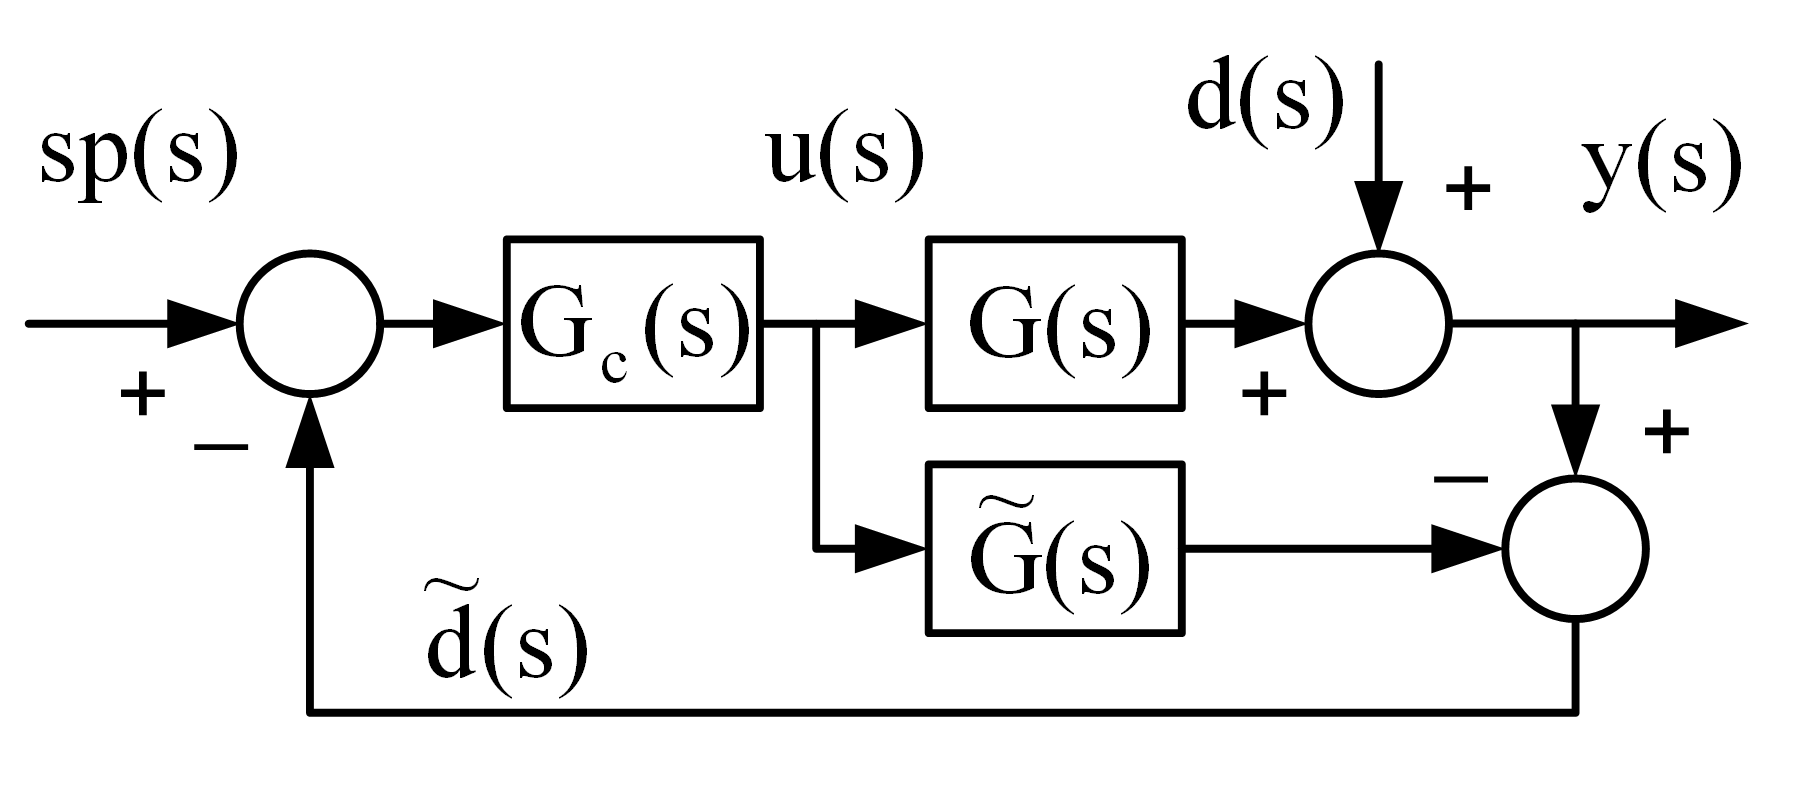
\includegraphics[width=7cm,height=3.5cm]{Appendix/fa1_b} \label{fa1a}}
\subfigure[Cl{\'a}sica]{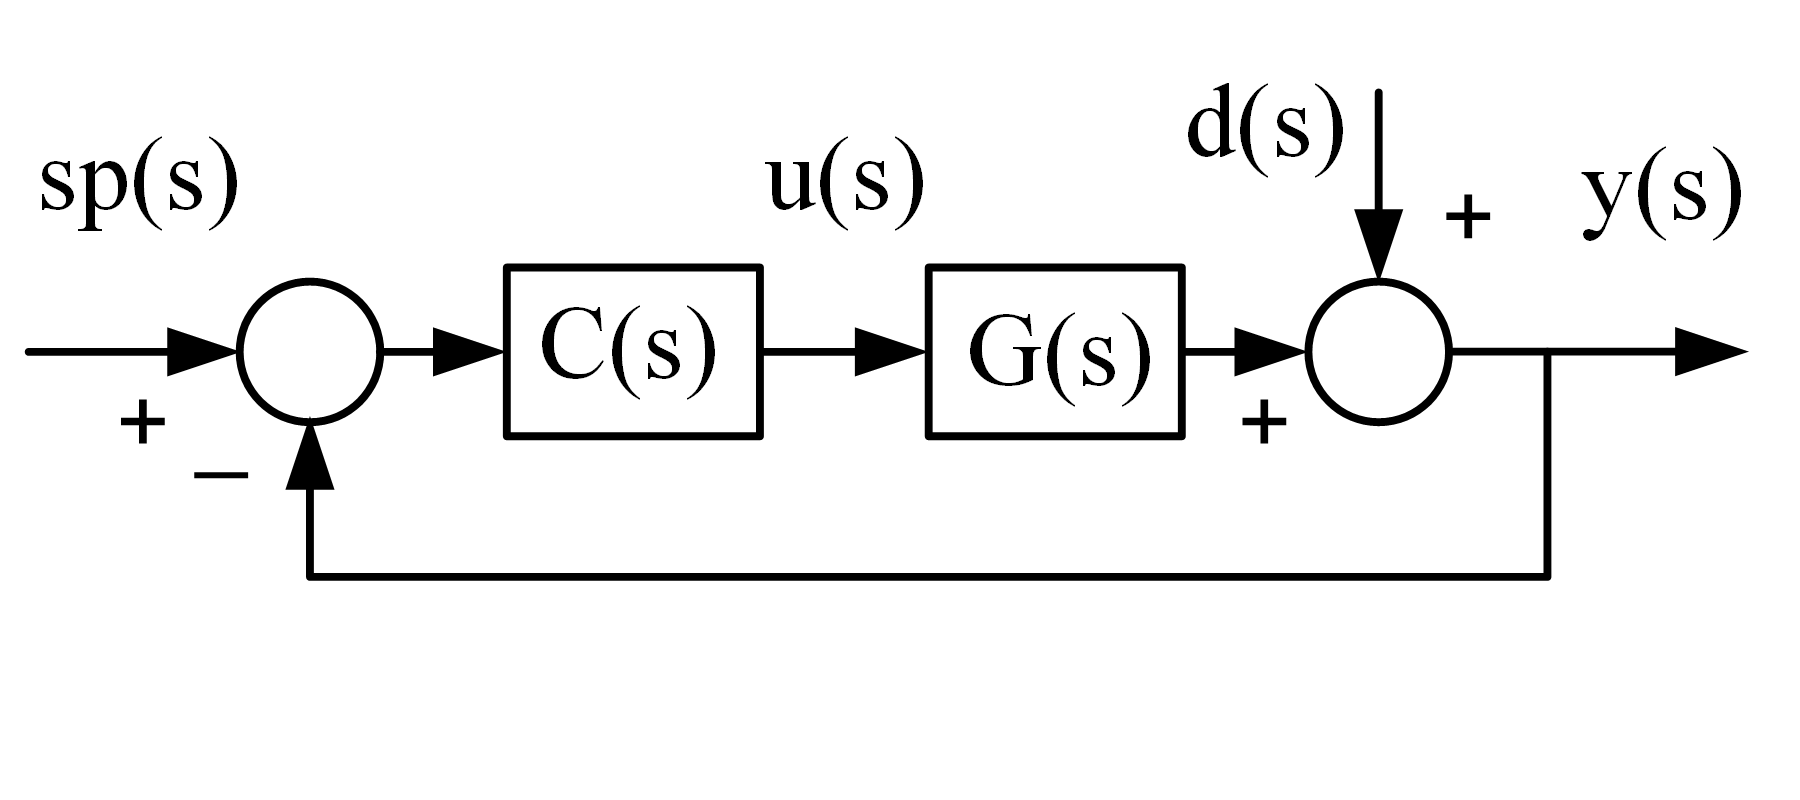
\includegraphics[width=7cm,height=3.5cm]{Appendix/fa1_a} \label{fa1b}}
\caption{Estructuras de control por realimentaci{\'o}n} \label{fa1}
\end{figure}
%--------------------------------------------------------------------------------------------------------------
\begin{equation}
    G_{c}(s)=\tilde{g}_{-}^{-1}(s)f_{lp}(s)
\end{equation}
donde $f_{lp}(s)$ es un filtro pasa bajos de orden espec{\'\i}fico de forma tal que $G_{c}(s)$ sea al menos una
funci{\'o}n propia. Mediante esta factorizaci{\'o}n $G_{c}(s)$ resulta f{\'\i}sicamente realizable.

Considerando entonces un modelo de primer orden de la forma $\tilde{G}(s)=k_{m}/(\tau_{m} s+1)$ y realizando
la factorizaci{\'o}n dicha anteriormente, $\tilde{g}_{+}(s)=1$ y $\tilde{g}_{-}(s)=k_{m}/(\tau_{m} s+1)$, se
puede ahora trabajar con algebra de bloque sobre la Fig. \ref{fa1a} y llegar a la estructura de control
cl{\'a}sica por realimentaci{\'o}n que se observa en la Fig. \ref{fa1b}, donde:
\begin{equation}
    C(s)=\frac{G_{c}(s)}{1-\tilde{g}(s)g_{c}(s)}=\frac{\tilde{g}^{-1}_{-}(s)}{f^{-1}_{lp}(s)-\tilde{g}_{+}(s)}
\end{equation}
que considerando ahora la factorizaci{\'o}n realizada y la transferencia del filtro $f_{lp}(s)=1/(\tau_{f}
s+1)$, el controlador resultante tiene la forma
\begin{equation}\label{ea_28}
    C(s)=\frac{\tau_{m} s +1}{k_{m}\tau_{f} s}=\frac{\tau_{m}}{k_{m}\tau_{f}}\left[1+\frac{1}{\tau_{m} s}\right]
\end{equation}
que es justamente la estructura de un controlador cl{\'a}sico PI. Es decir, se puede realizar el ajuste de este
controlador teniendo un modelo confiable de primer orden del proceso y los par{\'a}metros de un filtro pasa
bajos de primer orden. De esta forma la ganancia proporcional del controlador es calculada como
$\tau_{m}/k_{m}\tau_{f}$ y la constante de tiempo integral como $\tau_{m}$.

Cuando estamos en presencia de un modelo perfecto $\tilde{G}(s)=G(s)$ la constante de tiempo del filtro pasa
bajos puede seleccionarse libremente. En la pr{\'a}ctica raramente se obtiene un modelo perfecto del proceso,
generalmente puede aproximarse el comportamiento con modelos que poseen un rango de validez en un entorno
frecuencial de trabajo.

Un proceso puede ser satisfactoriamente modelado en la pr{\'a}ctica mediante un modelo de primer orden con
retardo de la forma $G(s)=k_{m}e^{-\xi s}/(\tau_{m} s+1)$. Recordando que para derivar la ec. \ref{ea_28} se
utiliz{\'o} un modelo de primer orden sin informaci{\'o}n del retardo $\tilde{g}_{+}(s)=1$ (se asumi{\'o} una
aproximaci{\'o}n del retardo Pad{\'e} de orden cero, $e^{-\xi s}=1$), la estrategia de CBMI permite cuantificar la
validez de dicho modelo y delimitar el rango de frecuencias efectivo del sistema a lazo cerrado.

Para analizar el problema de utilizar una aproximaci{\'o}n Pad{\'e} de orden cero se define la \textit{funci{\'o}n de
error multiplicativo de norma acotada}, $|e_{m}(s)|$, donde
\begin{equation}
    e_{m}(s)=\frac{G(s)-\tilde{G}(s)}{\tilde{G}(s)}
\end{equation}

Generalmente $|e_{m}(s)|$ posee un valor que aproxima o supera la unidad para frecuencias altas. Evaluando
as{\'\i} $|e_{m}(\omega)|=1$ resulta que $\omega\cong 1/\xi$ generando un l{\'\i}mite frecuencial de validez para el
modelo. Para un rango operacional de $\omega>1/\xi$ no puede garantizarse la robustez a incertidumbres
multiplicativas. Adem{\'a}s, en la estrategia de CBMI la respuesta a lazo cerrado del sistema resulta
proporcional a la constante de tiempo del filtro $\tau_{f}$ (es decir $1/\tau_{f}=\omega$). En este
contexto, se puede obtener un dise{\~n}o conservativo si se selecciona $\tau_{f}> \xi$.

Teniendo en cuenta lo expresado hasta aqu{\'\i}, se puede entonces utilizar la informaci{\'o}n que suministra el
SDDEF respecto del retardo identificado y redise{\~n}ar los par{\'a}metros del controlador en l{\'\i}nea; considerando la
condici{\'o}n $\tau_{f}> \xi$ del error cometido y la ecuaci{\'o}n de dise{\~n}o \ref{ea_28}.

\section{Control en avance (feedforward control)}\label{A_6}
El control en avance (CEA) puede idealmente eliminar por completo el efecto de las perturbaciones medidas en
las salidas del proceso. Incluso cuando existen errores de modelado el CEA puede reducir el efecto de dichas
perturbaciones mejor que una estrategia de realimentaci{\'o}n solamente.

Los beneficios econ{\'o}micos del CEA pueden provenir de un menor costo operativo y/o incrementar la venta de
productos por mejoras en su calidad. Generalmente el CEA trabaja en conjunto con una estrategia de control
por realimentaci{\'o}n. Este {\'u}ltimo tiene por objeto realizar el seguimiento de la pol{\'\i}tica de referencia y
rechazar perturbaciones no medidas que siempre est{\'a}n presentes en proceso reales.

En la Fig. \ref{fa2} se puede observar la cl{\'a}sica estructura de un control por realimentaci{\'o}n (PI) actuando
en conjunto con un controlador en avance (CEA). Se puede entonces escribir la funci{\'o}n de transferencia entre
salida $y$ y  perturbaci{\'o}n medida $d$ como
% Figure-------------------------------------------------------------------
\begin{figure}[t]
\centering
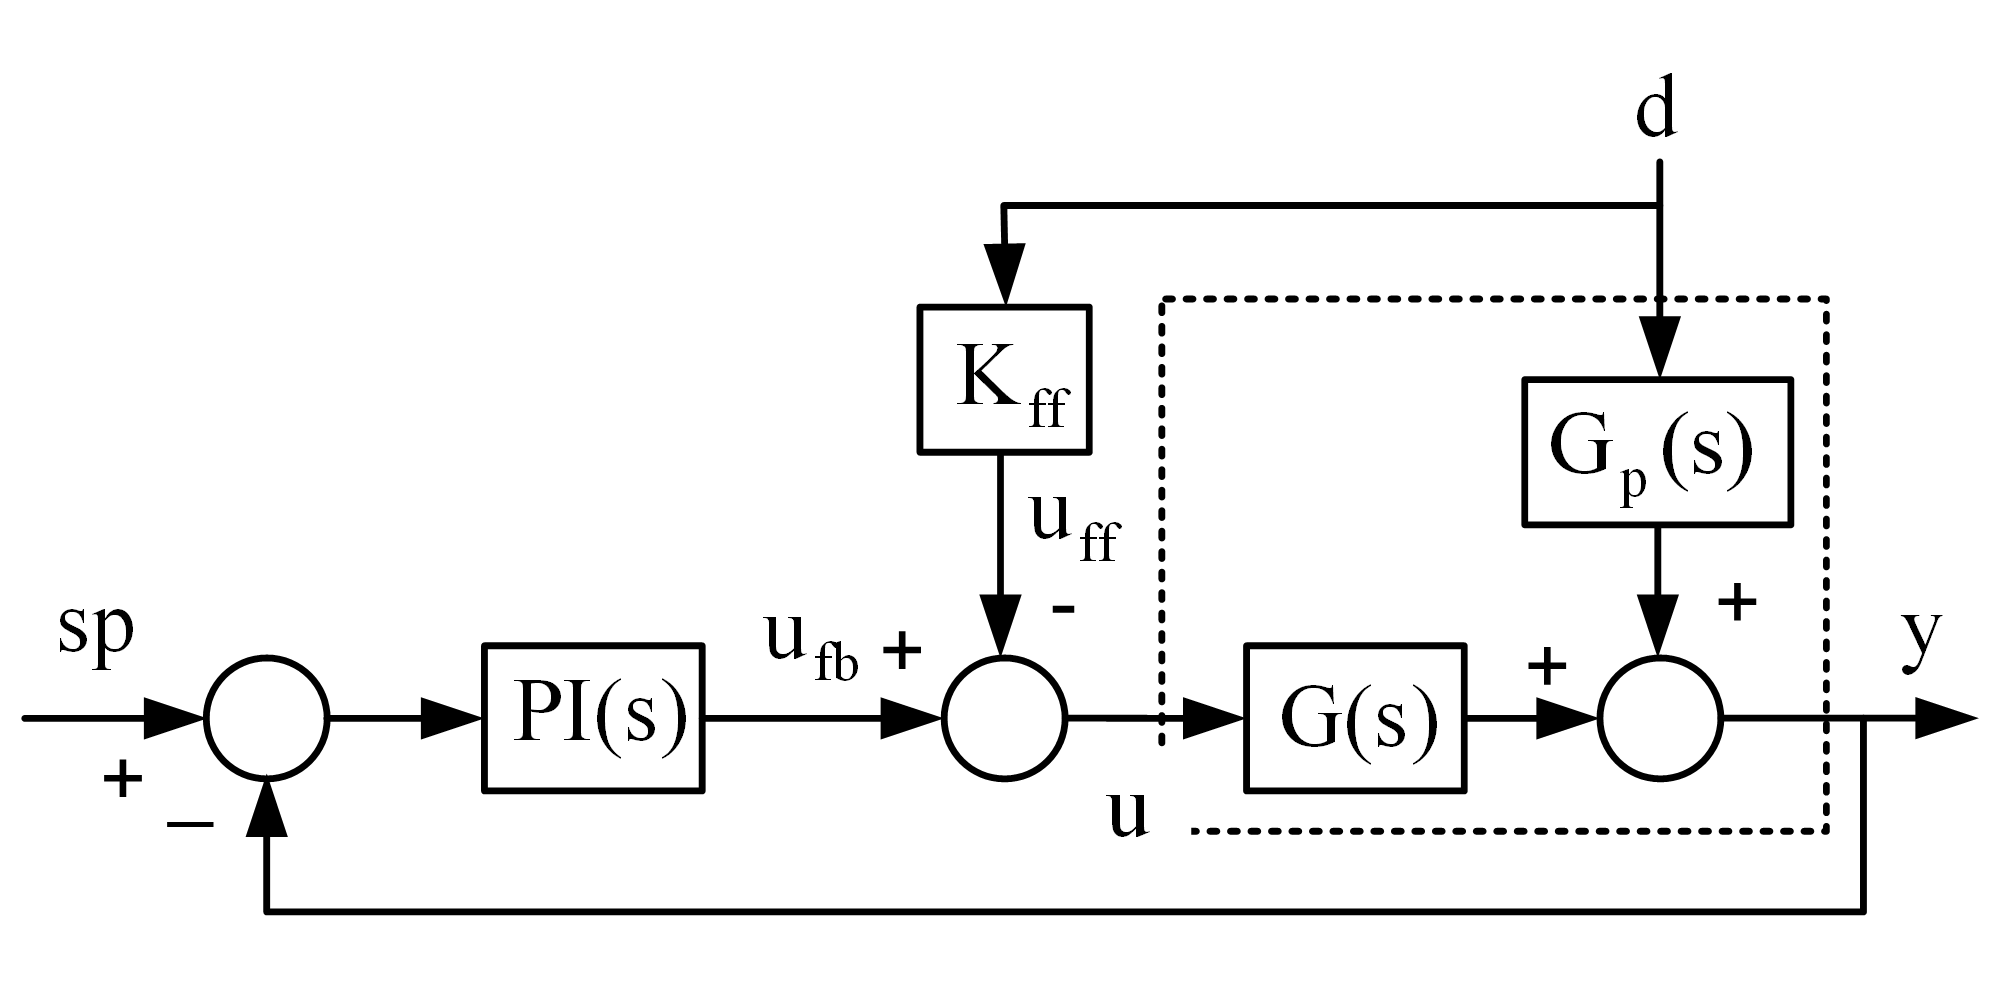
\includegraphics[width=11cm,height=6cm]{Appendix/fa2}
\caption{Estructura de control en avance (feedforward control)} \label{fa2}
\end{figure}
%-------------------------------------------------------------------------
\begin{equation}
   \frac{y(s)}{d(s)}=\frac{G_p(s)-K_{ff}(s)G(s)}{1+PI(s)P(s)}
\end{equation}
claramente se observa que si la perturbaci{\'o}n medida no debe influenciar la salida del proceso entonces se
debe cumplir que
\begin{equation}
   G_p(s)-K_{ff}(s)G(s)=0
\end{equation}
un c{\'a}lculo aproximado de dicho controlador puede realizarse considerando los modelos del proceso
$\tilde{G}(s)$ y $\tilde{G}_p(s)$ resultando en
\begin{equation}
   K_{ff}(s)=\tilde{G}^{-1}(s)\tilde{G}_p(s)
\end{equation}
teniendo en cuenta que el modelo $\tilde{G}(s)$ no contenga retardos ni ceros no m{\'\i}nima fase.
